\documentclass{standalone}   % change from article to standalone



% translate with >> pdflatex -shell-escape <file>

% This file is an extract of the PGFPLOTS manual, copyright by Christian Feuersaenger.
% 
% Feel free to use it as long as you cite the pgfplots manual properly.
%
% See
%   http://pgfplots.sourceforge.net/pgfplots.pdf
% for the complete manual.
%
% Any required input files (for <plot table> or <plot file> or the table package) can be downloaded
% at
% http://www.ctan.org/tex-archive/graphics/pgf/contrib/pgfplots/doc/latex/
% and
% http://www.ctan.org/tex-archive/graphics/pgf/contrib/pgfplots/doc/latex/plotdata/

\usepackage{pgfplots}
\pgfplotsset{compat=newest}

\pagestyle{empty}

\begin{document}
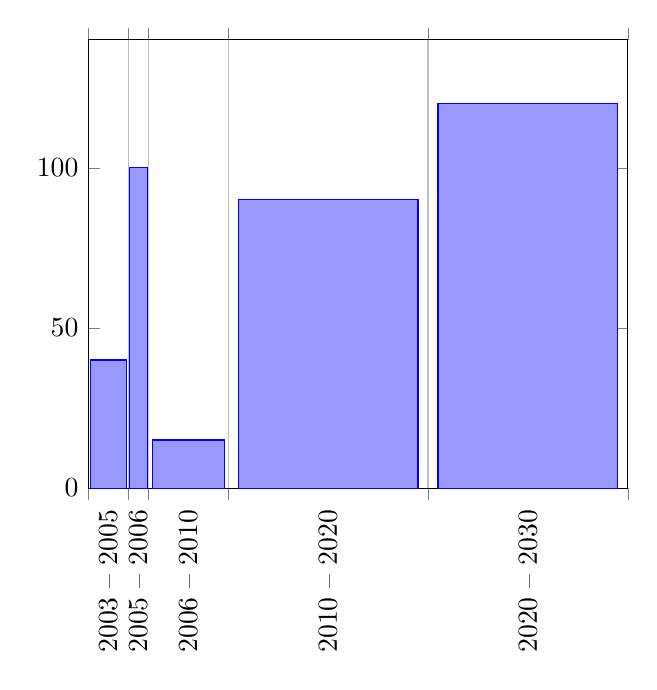
\begin{tikzpicture}
	\begin{axis}[
		ybar interval=0.90,    % separation between bars
		x tick label as interval,
		xmin=2003,xmax=2030,
		ymin=0,ymax=140,
		xticklabel={
			$\pgfmathprintnumber{\tick}$
			-- $\pgfmathprintnumber{\nexttick}$},
		xtick=data,
		x tick label style={
			rotate=90,anchor=east,
			/pgf/number format/1000 sep=}
		]
		
		\addplot[draw=blue,fill=blue!40!white]
		coordinates
		{(2003,40) (2005,100) (2006,15) 
			(2010,90) (2020,120) (2030,3)};
	\end{axis}
\end{tikzpicture}
\end{document}
